\iffalse

Nico Casale
Cody Orazymbetov
Chekad Sarami

ECE 592 Project 1

\fi

\documentclass[]{../../ncmathy}

\begin{document}
	
	\subsection{Part A: pdf of a Gaussian Mixture}
		The pdf of a mixture Gaussian source is given by the following steps. Using the example given in class, where there are two classes, blue and red, we have
		\begin{equation}
		f(x, Class = red) = \sum_{i=1}^{5} f_i(x, red)
		\end{equation}
		
		\begin{equation}
		f_i(\boldsymbol {x}) = \sum_{ri=1}^{5}(2\pi \boldsymbol{\Sigma})^{-\frac {1}{2}}\,e^{-\frac {1}{2}(\mathbf {x} -\boldsymbol{\mu_{ri} })'\boldsymbol{\Sigma}^{-1}(\mathbf{x} - \boldsymbol{\mu_{ri}})}
		\end{equation}

		\begin{equation}
		f(x, Class = blue) = \sum_{i=1}^{5} g_i(x, blue)
		\end{equation}

		\begin{equation}
		g_i(\boldsymbol {x}) = \sum_{bi=1}^{5}(2\pi \boldsymbol {\Sigma })^{-\frac {1}{2}}\,e^{-\frac {1}{2}}(\mathbf{x} - \boldsymbol{\mu_{bi}})'\boldsymbol{\Sigma}^{-1}(\mathbf{x} -\boldsymbol{\mu_{bi}})
		\end{equation}
	
	\subsection{Part B: Posterior Probability}
	Assuming equiprobable classes red and blue, the posterior probability is given as:
	\begin{align*}
	Pr(class = red|x) &= \frac{f(x, Class = red)}{f(x, Class = red) + f(x, Class = blue)}\\
	\numberthis
	\end{align*}
	
	\subsection{Part C: Code for Optimal Decision Regions}
		\subsubsection{Outline of application of Bayes decision region}
	From the above equation, given coordinates we can calculate the probability of red or blue class assuming that we have 2 clusters of blue and red color. If they are both normally distributed with equal covariance matrix, then we can exploit Bayesian decision boundary which compares probabilities of both colors at a given coordinate and selects the one with higher probability. Mathematically, for a given \textbf{x} if 
	\begin{equation}
	Pr(class = red|x)  > Pr(class = blue|x)
	\end{equation}
	then we decide that our data point belongs to red color. 
		\subsubsection{Results with Bayes decision boundary}
	If we look our decision boundary in 2D, then we should get a linear line separating the two class.  
	
	\begin{figure}[H]
		\centering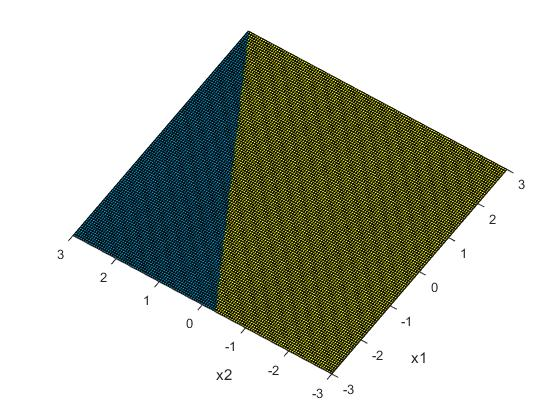
\includegraphics[width=0.6\textwidth]{2dbayes}
		\caption{Bayes Classifier with same covariance matrix in 2D.}
	\end{figure}
	
	In 3D we should observe overlap of two Gaussian distributions and we should select the most probable one when one decreases in pdf while another increases in pdf.
		\begin{figure}[H]
				\centering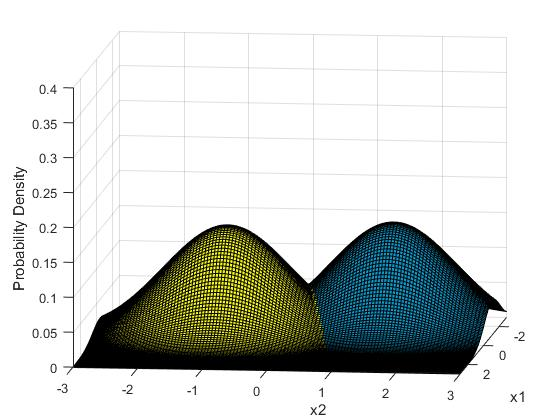
\includegraphics[width=0.6\textwidth]{3dbayes}
				\caption{Bayes Classifier with same covariance matrix in 3D.}
		\end{figure}

	\subsection{Part D: Quadratic Discriminant Analysis (QDA)}
		In QDA, we do not assume that the class covariances are equal. This leads to a quadratic decision boundary, as we will show in the following sections.
		
		\subsubsection{pdf for QDA}
			The pdf of the two classes, where each is composed of a single Gaussian component can be represented as the sum of two multivariate Gaussian distributions:
			
			\begin{equation}
				f_{\mathbf X}(x_1, x_2) = \sum_{k=1}^2\sqrt{|2\pi\boldsymbol\Sigma_k|}^{-1}\exp\left(-\frac{1}{2}({\mathbf x}-{\boldsymbol\mu_k})^\mathrm{T}{\boldsymbol\Sigma_k}^{-1}({\mathbf x}-{\boldsymbol\mu_k})\right)
			\end{equation}		
			Note that $\boldsymbol\Sigma_k$ is positive definite and has a non-zero determinant for each class $C_k$ in $k = [1,2]$ (in the square root.) $\mu_k$ is the mean of each class.
		
		\subsubsection{Posterior Probability for QDA}
			The posterior probability for QDA is derived by first using Bayes' Theorem as
			
			\begin{equation}
			p(C_k|x) = \frac{p(C_k)p(x|C_k)}{p(x)}
			\label{eq:bayes}
			\end{equation}
			
			Where $x$ is the vector of features. In the 2-D case, there are only 2 features, $x_1$ and $x_2$. The numerator of Eq. (\ref{eq:bayes}) is equivalent to the joint probability model, $p(C_k,x_1,x_2)$, which is equivalent to
			
			\begin{align*}
				p(C_k,x_1,x_2) &= p(x_1, x_2, C_k)\\
				&= p(x_1 | x_2, C_k)p(x_2,C_k)\\
				&= p(x_1 | x_2, C_k)p(x_2|C_k)p(C_k)\\
				\numberthis
			\end{align*}
			
			Assuming that each feature (in the x and y dimension) is independent, 
			
			\begin{equation}
			p(C_k|x_1,x_2) \varpropto p(C_k,x_1,x_2) \varpropto p(C_k)p(x_1|C_k)p(x_2|C_k)
			\end{equation}
			
			Incorporating the probability of x,
			
			\begin{equation}
				p(C_k|x_1,x_2) = \frac{1}{p(x)}p(C_k)p(x_1|C_k)p(x_2|C_k)
				\label{eq:bayes1}
			\end{equation}
			
			%Note that $p(x_2|C_k) = p(x_2,C_k)p(C_k)$, and multiplying Eq. (\ref{eq:bayes1}) by $\frac{p(C_k)}{p(C_k)}$,
			
			%\begin{equation}
			%	p(C_k|x_1,x_2) = \frac{1}{p(C_k)p(x)}p(x_1,C_k)p(x_2,C_k)
			%\end{equation}
			
			Simplifying,
			
			\begin{align*}
				p(C_k|x) &= \frac{1}{p(x)}p(C_k)f_k(x)\\
				&= \frac{p(C_k)f_k(x)}{\sum_{k'=1}^{2}p(C_{k'})f_{k'}(x)}\\
				\numberthis
			\end{align*}
			
			The Bayesian classifier will choose the $C_k$ that maximizes the conditional probability $p(C_k|x)$. To see that the decision boundary is quadratic, consider the log-likelihood ratio of the two class pdf's:
			
			\begin{equation}
			\text{likelihood ratio} = \frac{ \sqrt{|2 \pi \Sigma_{k=1}|}^{-1} \exp \left( -\frac{1}{2}(x-\mu_{k=1})^T \Sigma_{k=1}^{-1} (x-\mu_{k=1}) \right) }{ \sqrt{|2 \pi \Sigma_{k=0}|}^{-1} \exp \left( -\frac{1}{2}(x-\mu_{k=0})^T \Sigma_{k=0}^{-1} (x-\mu_{k=0}) \right)} < t
			\end{equation}
			
			Where $t$ is the threshold where the numerator or denominator starts to be larger than the other. Taking the natural log of both sides,
			
			\begin{equation}
			(x- \mu_0)^T \Sigma_0^{-1} (x- \mu_0) + \ln|\Sigma_0| - (x- \mu_1)^T \Sigma_1^{-1} ( x- \mu_1) - \ln|\Sigma_1| \ > \ T
			\end{equation}
			
			Where $T = \ln(t)$. Note that the inequality flips because we divided by $-\frac{1}{2}$. Multiplying out,
			
			\begin{equation}
			x^T\Sigma_0^{-1}x - x^T\Sigma_1^{-1}x + x^T\Sigma_0^{-1}\mu_0 - x^T\Sigma_1^{-1}\mu_1 > T - \mu_0^T\Sigma_0^{-1}\mu_0 + \mu_1^T\Sigma_0^{-1}\mu_1 - \ln|\Sigma_0| + \ln|\Sigma_1|
			\end{equation}

			Note that the quadratic elements of this inequality are the two leftmost terms. 
			\\\\
			Sources:
			\begin{itemize}
				\item Dr. Baron's \href{https://courses.ncsu.edu/ece592/lec/059/supplements/supplement09152017.pdf}{supplement} on Bayesian Analysis.
				\item \href{https://en.wikipedia.org/wiki/Quadratic\_classifier}{Quadratic Classifiers on Wikipedia}
				\item \href{https://en.wikipedia.org/wiki/Linear\_discriminant\_analysis}{Linear Discriminant Analysis on Wikipedia}
				\item \href{https://en.wikipedia.org/wiki/Naive\_Bayes\_classifier}{Naive Bayes Classifiers on Wikipedia}
			\end{itemize}
		
		\subsubsection{Code for Optimal Decision Regions under QDA}
			The figure below illustrates the results of a Bayesian classifier without the assumption that the covariance between classes is equal. Under this premise, a quadratic decision boundary is needed to separate the two classes in such a way that $p(C_k|x)$ is maximized for each class.
			
			\begin{figure}[H]
			\centering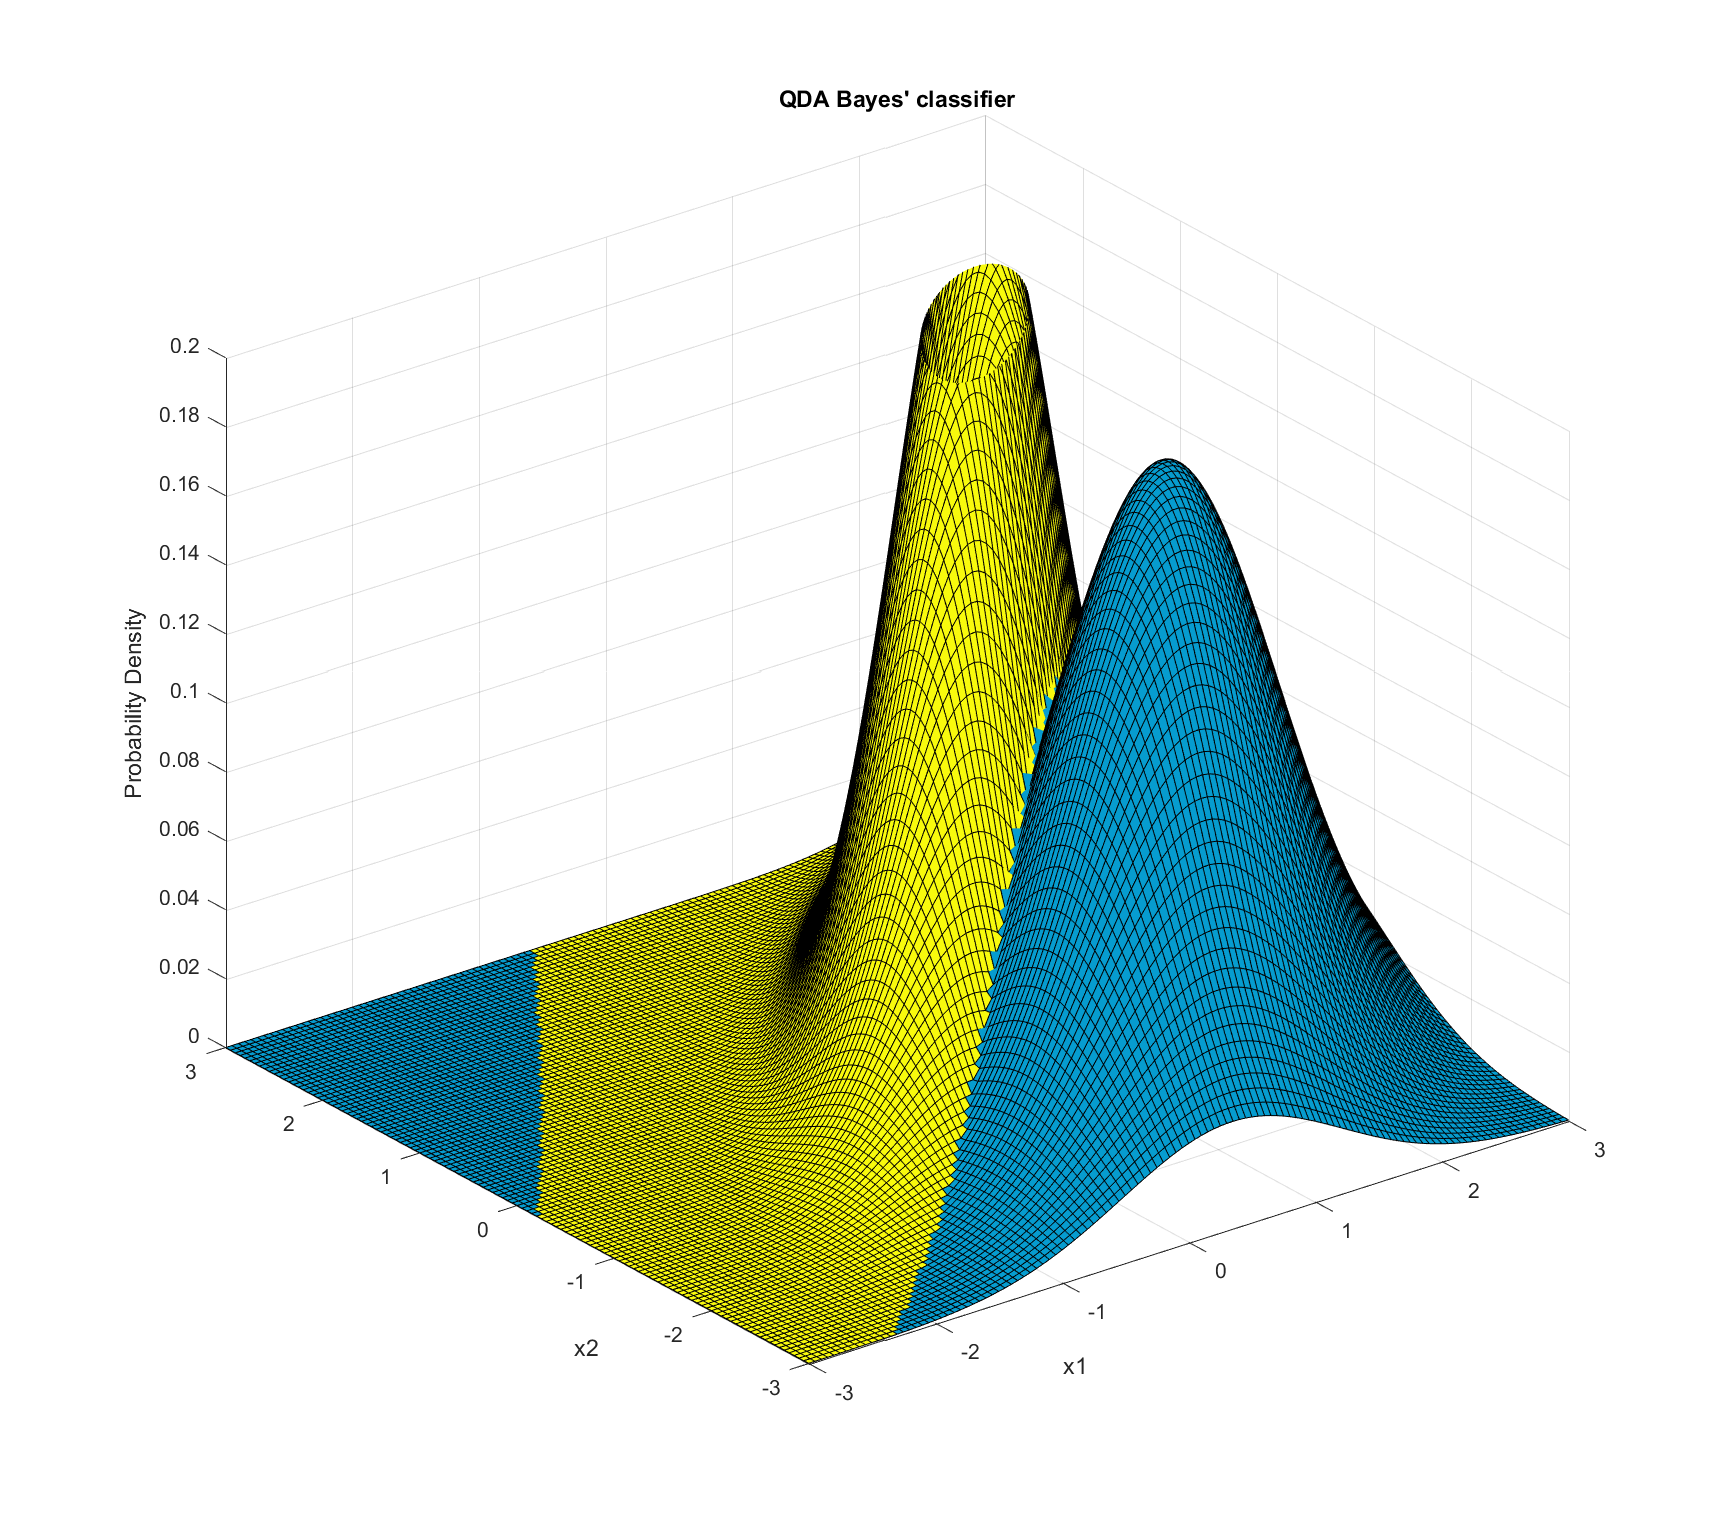
\includegraphics[width=0.6\textwidth]{qda_bayes1}
			\caption{Bayes Classifier with QDA.}
			\end{figure}

\end{document}